\documentclass{scrartcl}
\usepackage{graphicx}
\usepackage{amsmath}
\usepackage{listings}
\usepackage{mathtools}
\usepackage{physics}
\usepackage{siunitx}
\usepackage{tikz}
\usepackage{mathtools}
\usepackage{rotating}
\usepackage{hyperref}
\usepackage{fancyhdr}
\usepackage{float}

\pagestyle{fancy}
\fancyhf{}
\rhead{Jamie Grieser}
\lhead{Simulation Methods}
\rfoot{Page \thepage}

\definecolor{mygreen}{rgb}{0,0.6,0}
\definecolor{mygray}{rgb}{0.5,0.5,0.5}
\definecolor{mymauve}{rgb}{0.58,0,0.82}

\lstset{ 
	backgroundcolor=\color{white},   % choose the background color; you must add \usepackage{color} or \usepackage{xcolor}; should come as last argument
	basicstyle=\footnotesize,        % the size of the fonts that are used for the code
	breakatwhitespace=false,         % sets if automatic breaks should only happen at whitespace
	breaklines=true,                 % sets automatic line breaking
	captionpos=b,                    % sets the caption-position to bottom
	commentstyle=\color{mygreen},    % comment style
	deletekeywords={...},            % if you want to delete keywords from the given language
	escapeinside={\%*}{*)},          % if you want to add LaTeX within your code
	extendedchars=true,              % lets you use non-ASCII characters; for 8-bits encodings only, does not work with UTF-8
	frame=single,	                   % adds a frame around the code
	keepspaces=false,                 % keeps spaces in text, useful for keeping indentation of code (possibly needs columns=flexible)
	keywordstyle=\color{blue},       % keyword style
	language=Octave,                 % the language of the code
	morekeywords={*,...},            % if you want to add more keywords to the set
	numbers=left,                    % where to put the line-numbers; possible values are (none, left, right)
	numbersep=5pt,                   % how far the line-numbers are from the code
	numberstyle=\tiny\color{mygray}, % the style that is used for the line-numbers
	rulecolor=\color{black},         % if not set, the frame-color may be changed on line-breaks within not-black text (e.g. comments (green here))
	%showspaces=false,                % show spaces everywhere adding particular underscores; it overrides 'showstringspaces'
	showstringspaces=false,          % underline spaces within strings only
	showtabs=false,                  % show tabs within strings adding particular underscores
	stepnumber=2,                    % the step between two line-numbers. If it's 1, each line will be numbered
	stringstyle=\color{mymauve},     % string literal style
	tabsize=2,	                   % sets default tabsize to 2 spaces
	%title=\lstname                   % show the filename of files included with \lstinputlisting; also try caption instead of title
}

\begin{document}

\section*{Problem Sheet 6}
\subsection*{Exercise 1.1}
To derive the numeric form of the equation on the grid, we use the example given in the script with Dirichlet boundary condition:
\begin{equation}
	-D \dfrac{T_{i+1} - 2 T_{i} + T_{i-1}}{h^2} = \epsilon
\end{equation}
In matrix notation, this reads:
\begin{equation} \label{matrixeq}
	\begin{pmatrix}
	1& \\
	1&-2&1\\
	&&\ddots&\\
	&&1&-2&1\\
	&&&&1
	\end{pmatrix}
	\begin{pmatrix}
	T_1\\
	\vdots\\
	T_i\\
	\vdots\\
	T_{N}
	\end{pmatrix}
	=
	\begin{pmatrix}
	T_0\\
	-\dfrac{\epsilon h^2}{D}\\
	\vdots\\
	-\dfrac{\epsilon h^2}{D}\\
	T_0\\
	\end{pmatrix}
\end{equation}
Th following equation initializes the elements of the sparse matrix from \eqref{matrixeq} using three 1D arrays with N elements:
\begin{lstlisting}[title=Function to initialize the 3D array. Notice that the array for the diagonal part contains one element more than the off diagonal lower and upper part. The corresponding entry in the array is set to one but ignored in any further computation.,  language=Python, frame=single]
def initialize_matrix(N):
	diagonal = np.ones((N, 1))
	upper = np.ones((N, 1))
	lower = np.ones((N, 1))
	
	diagonal = np.multiply(diagonal, -2)
	diagonal[0] = 1
	diagonal[N-1] = 1
	lower[N-1] = 0
	upper[0] = 0
	return lower, diagonal, upper
\end{lstlisting}
The matrix multiplication with the sparse matrix is realized through:
\begin{lstlisting}[title=Function to multiply the given sparse matrix with a vector.,  language=Python, frame=single]
# Function to multiply a trigonal matrix and a vector
def trigonal_multiplication(lower, diagonal, upper, vector):
	result = np.zeros((N, 1))
	result[0] = diagonal[0] * vector[0]
	result[N-1] = diagonal[N-1] * vector[N-1]
	for i in range(1, N-1):
		result[i] = lower[i] * vector[i-1] + diagonal[i] * vector[i] + upper[i] * vector[i+1]
	return result
\end{lstlisting}
Testing this algorithm with an input vector equal to one yields the output:
\begin{lstlisting}[title=,  language=Python, frame=single]
[[1.][0.][0.][0.][0.][0.][0.][0.][1.]]
\end{lstlisting}
This is exactly what we would expect. Thus, we are fine to assume that the algorithm works correctly.
We now turn to the implementation of the forward-elimination backward-substitution algorithm. We splitted this into two parts:
\begin{lstlisting}[title=Function for the forward elimination step.,  language=Python, frame=single]
# Function that implements the forward-elimination, backward-substitution algorithm
def forward_elimination(lower, diagonal, upper, b):
	for i in range(0, N-2):
		if diagonal[i] > 0:
			m = (-1) * np.abs(lower[i+1]/diagonal[i])
		else:
			m = np.abs(lower[i + 1] / diagonal[i])
		lower[i+1] = lower[i+1] + m * diagonal[i]
		diagonal[i+1] = diagonal[i+1] + m * upper[i]
		b[i+1] = b[i+1] + m * b[i]
	return diagonal, b
\end{lstlisting}
This function only returns the diagonal and the b-part. The lower will  be equal to zero after performing the procedure while the upper part will still have the same shape. Thus they are not returned by the algorithm.
Now we turn to the backward-substitution step:
\begin{lstlisting}[title=Function for the backward substitution step.,  language=Python, frame=single]
# Function that implements the backward-substitution step
# The output vector contains the values for T_i
def backward_substitution(diagonal, b):
	result = np.zeros((N, 1))
	result[N-1] = b[N-1]
	result[0] = b[0]
	for i in range(2, N):
		result[N-i] = (b[N-i] - result[N-i+1])/diagonal[N-i]
	return result
\end{lstlisting}
To run the algorithm, we use:
\begin{lstlisting}[title=Runs the forward-backward algorithm and plots the result and also calculates the residual.,  language=Python, frame=single]
# Function to run the full algorithm
def run_matrix_algorithm():
	l, d, u = initialize_matrix(N)
	b = initialize_b(T_0)
	a, b = forward_elimination(l, d, u, b)
	y = backward_substitution(a, b)
	
	# Verify solution and calculate residual
	l, d, u = initialize_matrix(N)
	b = initialize_b(T_0)
	print('Residual:', trigonal_multiplication(l, d, u, y) - b)
	
	x = create_x_array()
	plt.plot(x, y, 'k--')
\end{lstlisting}
The plot of the solution looks like:
\begin{figure}[!h]
	\centering
	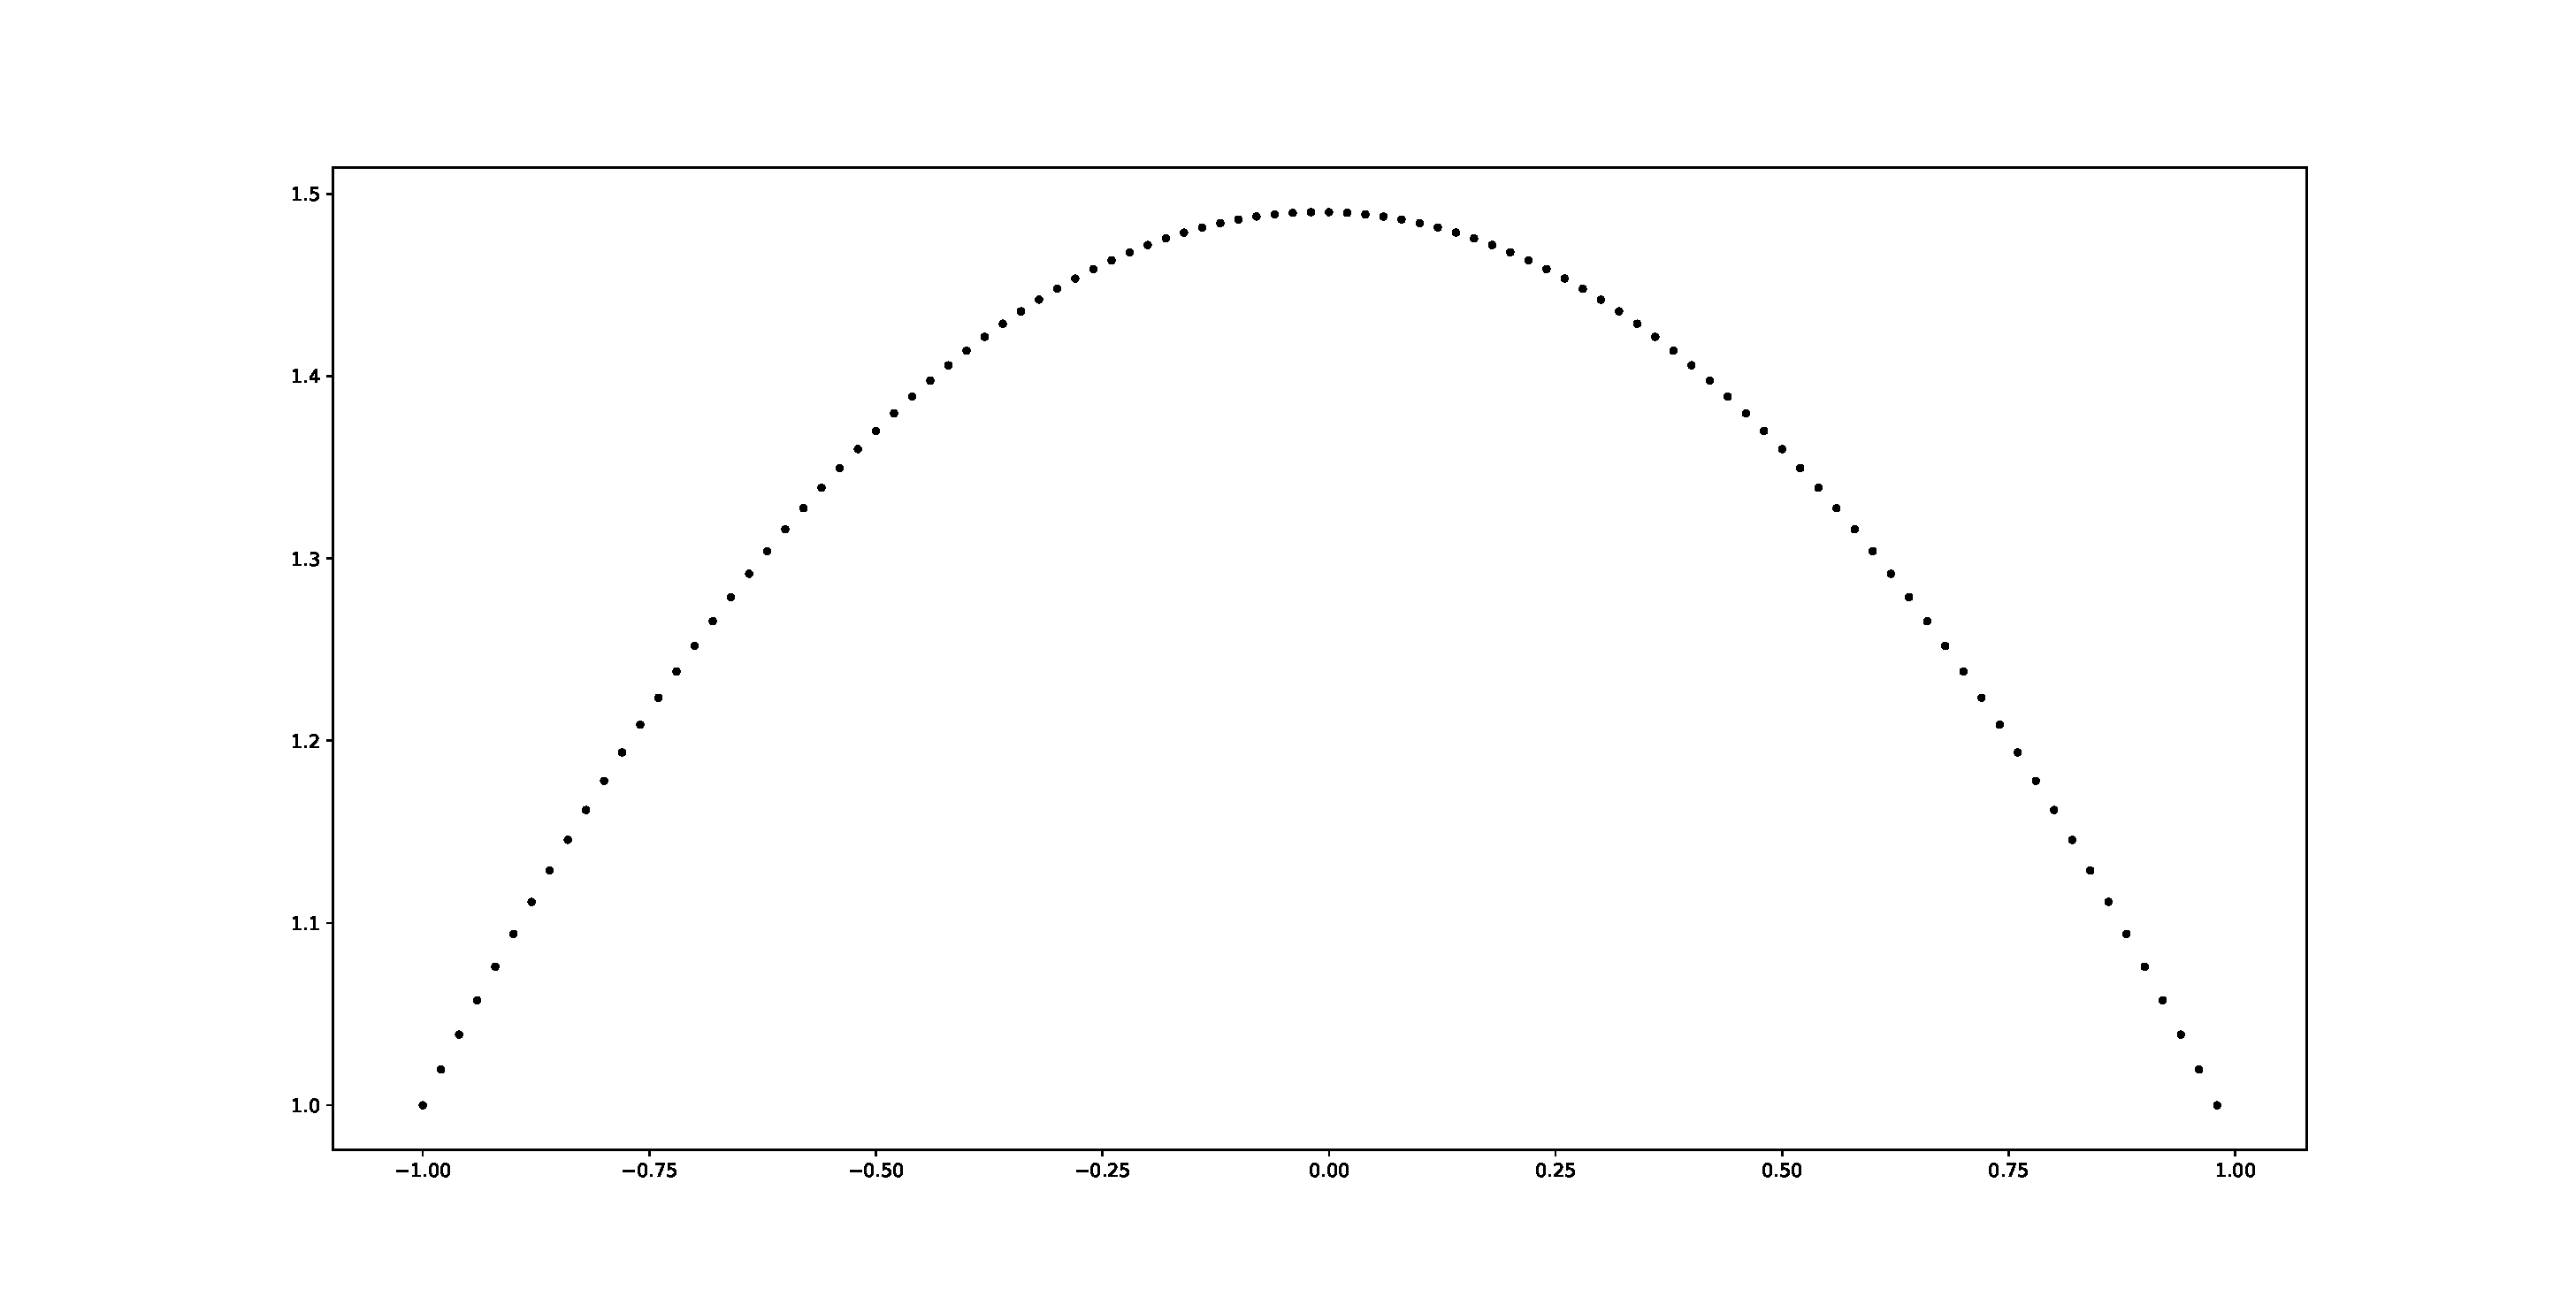
\includegraphics[width=0.8\linewidth]{Plots/forwardbackward100.eps}
	\caption{Plot of the solution for \(N=100\)}
	\label{fig:forwardbackwardplot100}
\end{figure}
This looks quite similar to a parabola, which is what we would expect as a solution to the partial differential equation.
The residual does not vanish for the the given problem. Instead it is of order \( 10^{-16} \) to \( 10^{-17} \). This is probably due to finite machine precision when multiplying large numbers with small numbers.
Here we can see the same result for \(N=1000\):
\begin{figure}[!h]
	\centering
	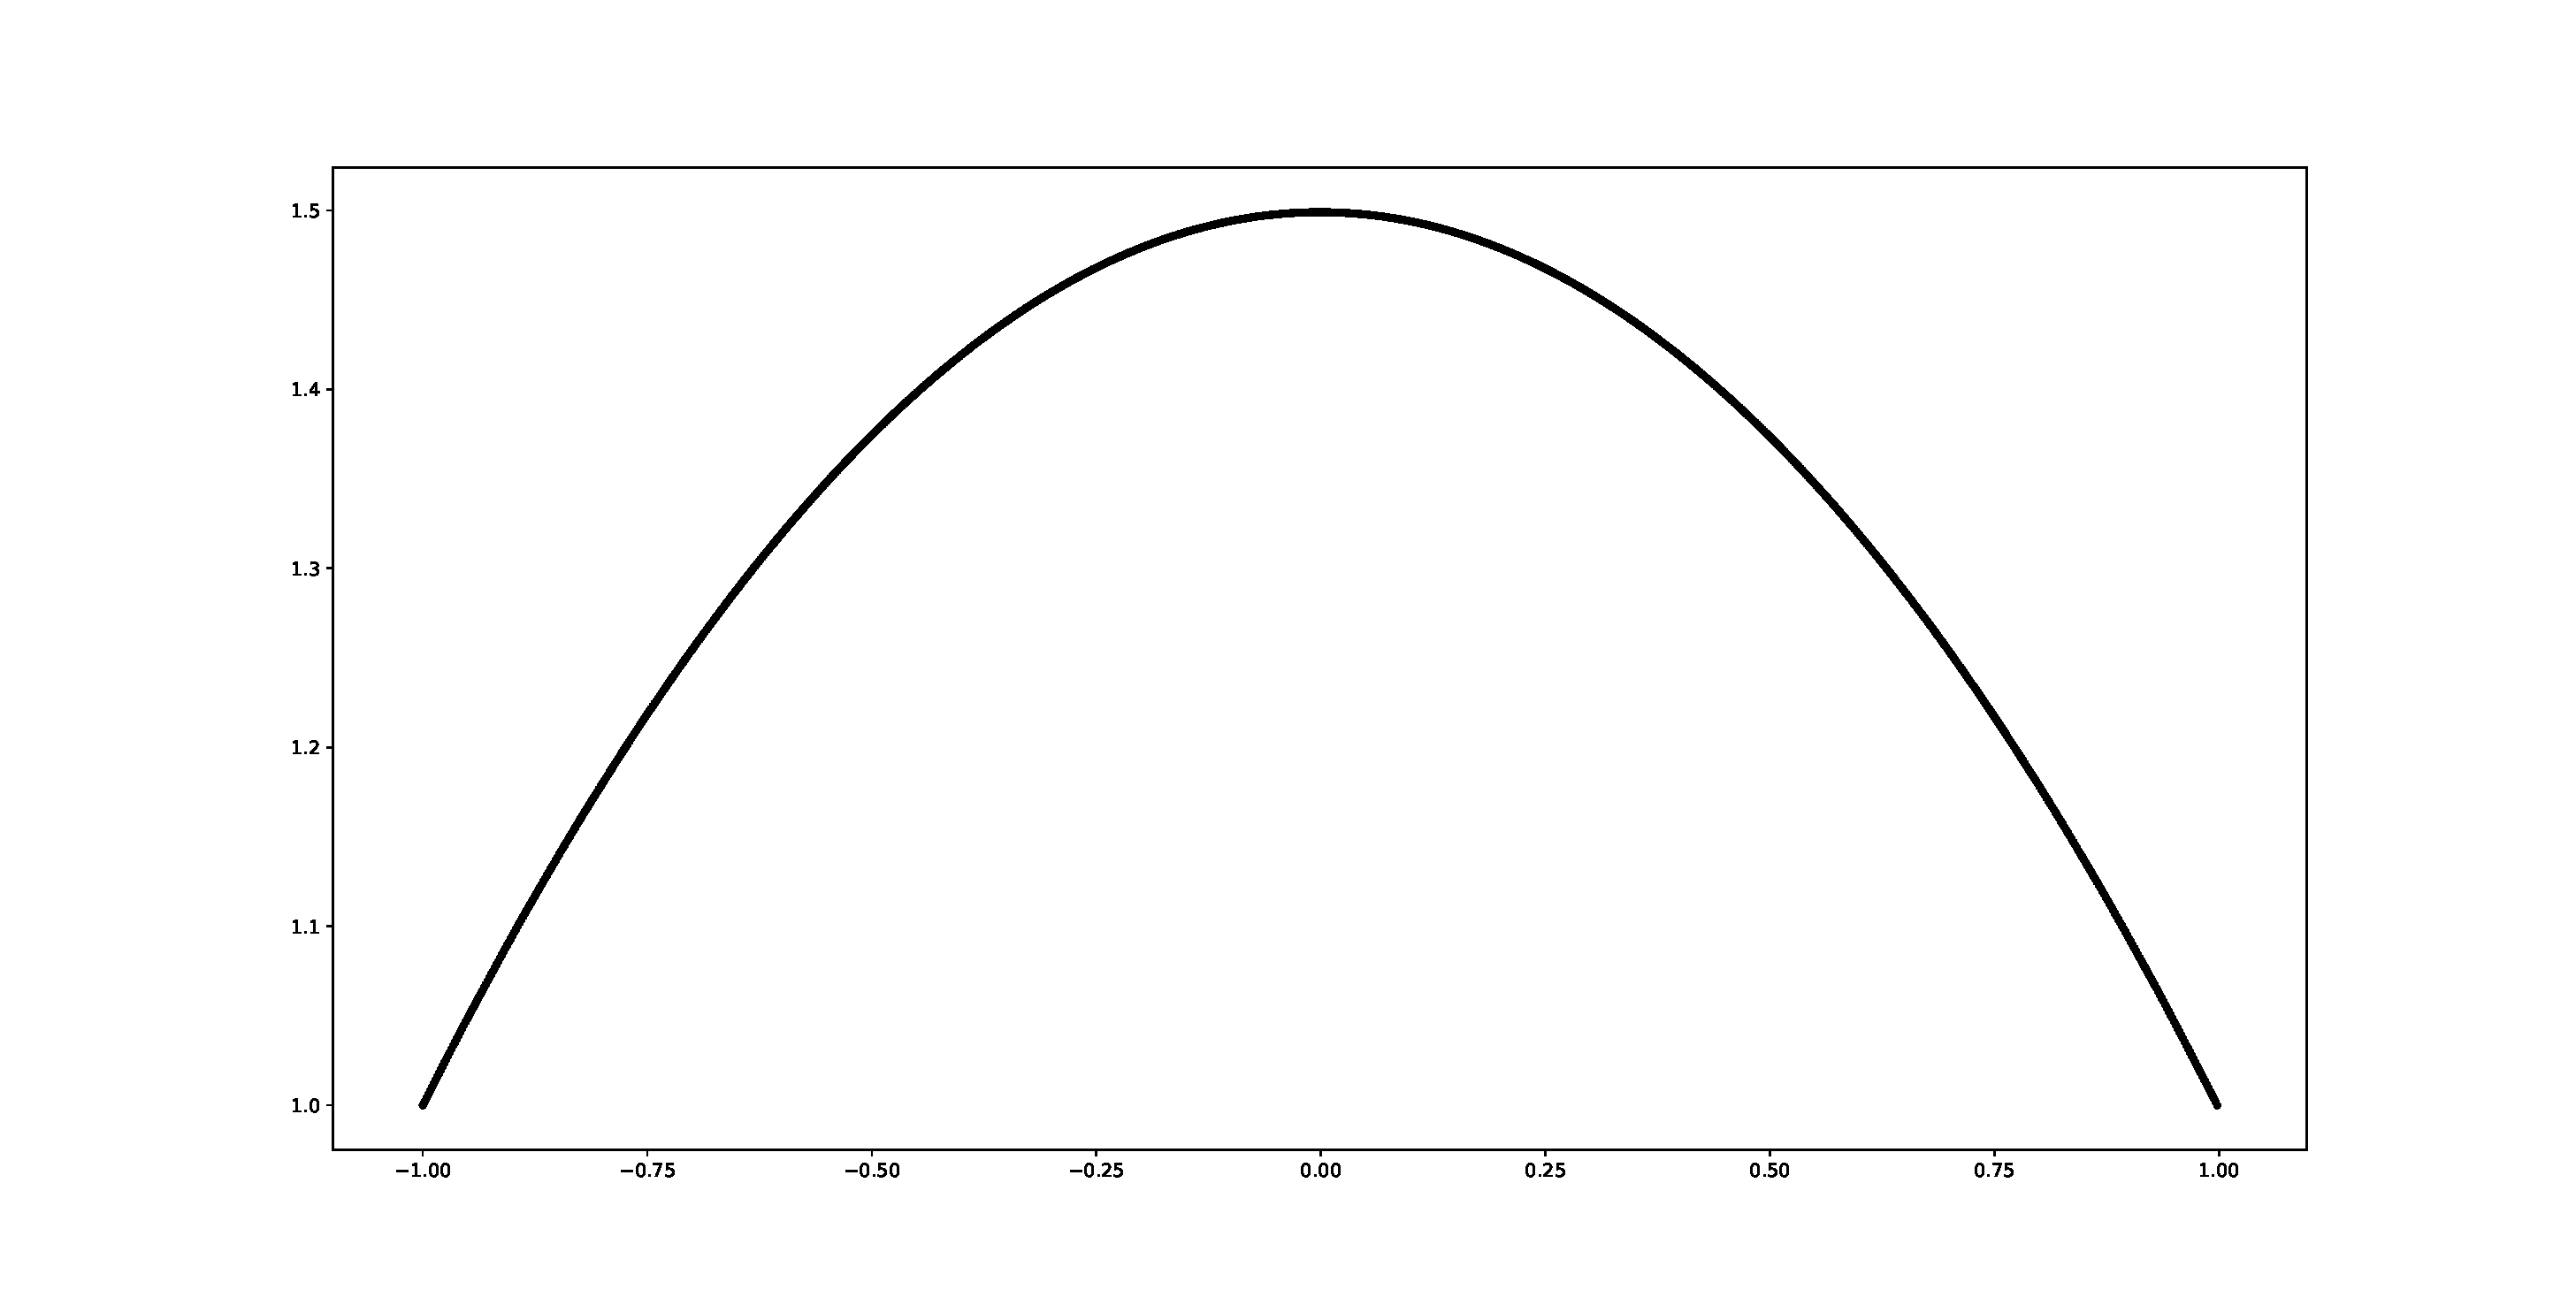
\includegraphics[width=0.8\linewidth]{Plots/forwardbackward1000.eps}
	\caption{Plot of the solution for \(N=1000\)}
	\label{fig:forwardbackwardplot1000}
\end{figure}

We see that the solution is much smoother for higher numbers of \( N \). \\\\Next, we implement the Jacobi iteration.
To do this we start by writing a function that does one Jacobi step per call:
\begin{lstlisting}[title=Function that performs one Jacobi step.,  language=Python, frame=single]
# Function that implements a Jacobi iteration
def jacobi_step(lower, diagonal, upper, x, b):
	zero = np.zeros((N, 1))
	p = trigonal_multiplication(lower, zero, upper, x)
	x = trigonal_multiplication(zero, 1./diagonal, zero, b + p)
	return x
\end{lstlisting}
To run this function, we use the following piece of code:
\begin{lstlisting}[title=Function to perform several Jacobi steps and plots the result for each step.,  language=Python, frame=single]
# Function to run the full jacobi algorithm
def run_jacobi_algorithm(steps):
	x = create_x_array()
	l, d, u = initialize_matrix(N)
	b = initialize_b(T_0)
	y = np.zeros((N, 1))
	for i in range(0, steps):
		y = jacobi_step((-1) * l, d, (-1) * u, y, b)
		plt.plot(x, y)
\end{lstlisting}
Result for \( N=8 \) grid points and \(30\) steps:
\begin{figure}[H]
	\centering
	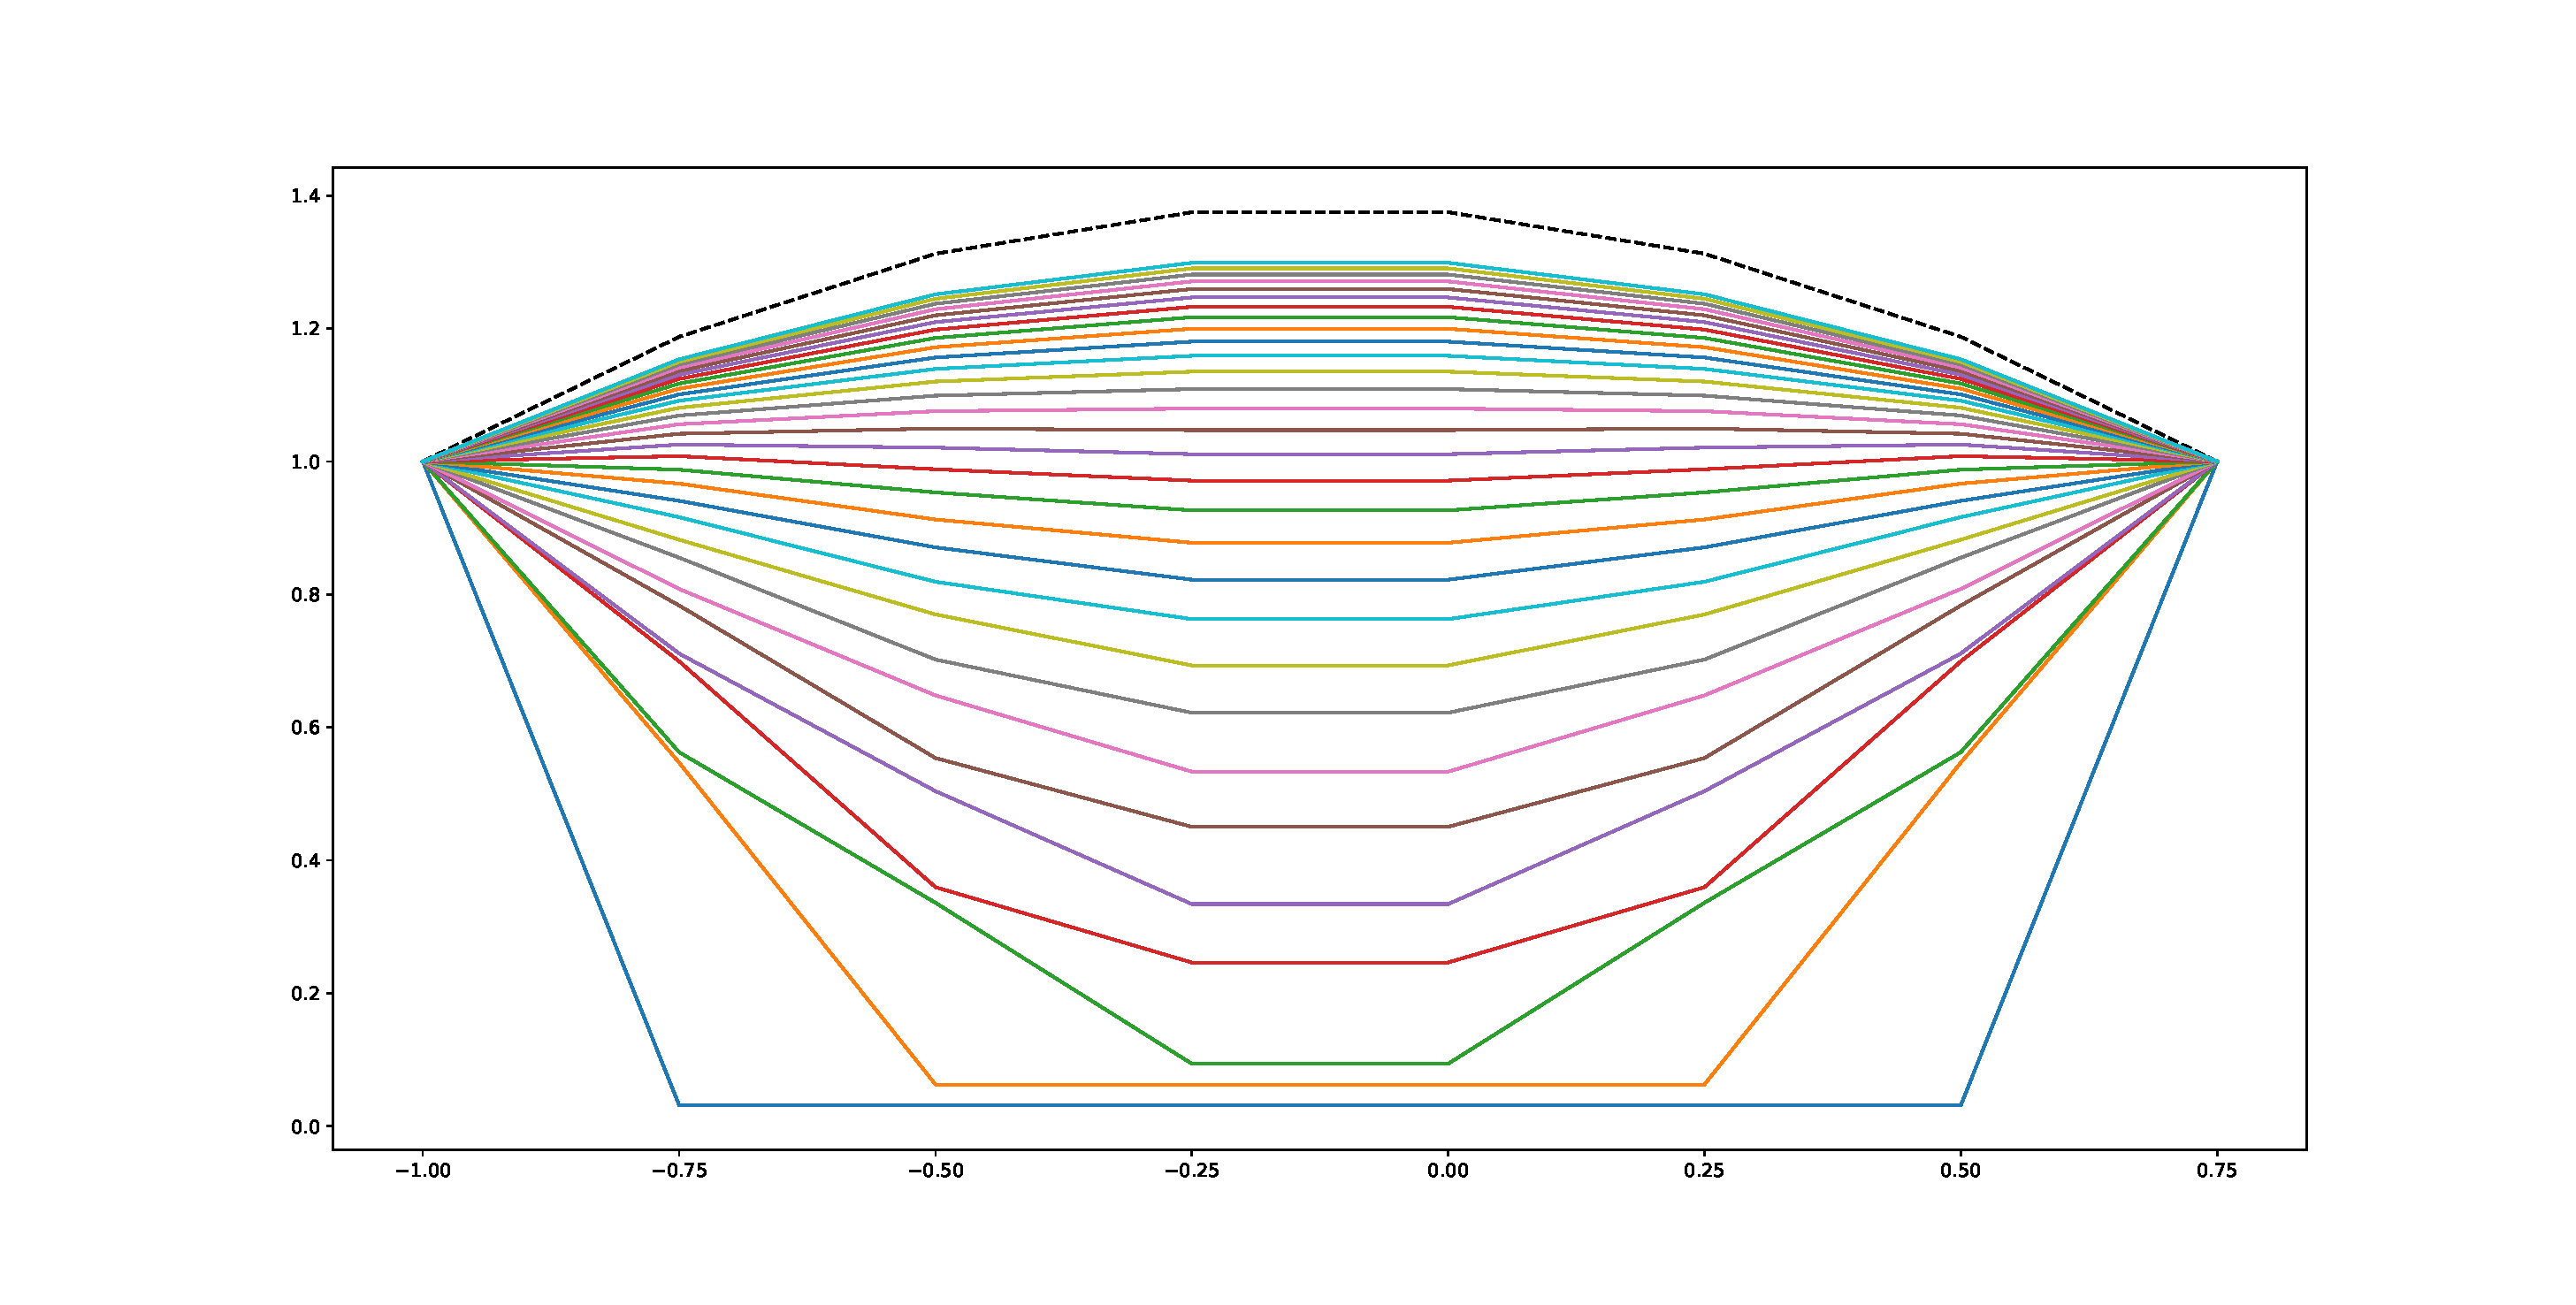
\includegraphics[width=1.1\linewidth]{Plots/Jacobi_Comparison.eps}
	\caption{Jacobi iteration for \(30\) steps and \( N=100 \). The black, dotted line indicates the solution obtained form he previous algorithm.}
	\label{fig:Jacobi_Comparison}
\end{figure}
We see that in the first few steps, that the information is propagating from the boundaries to the middle. After some time a parabola arises.
We now compute the same for \( N=100 \):
\begin{figure}[H]
	\centering
	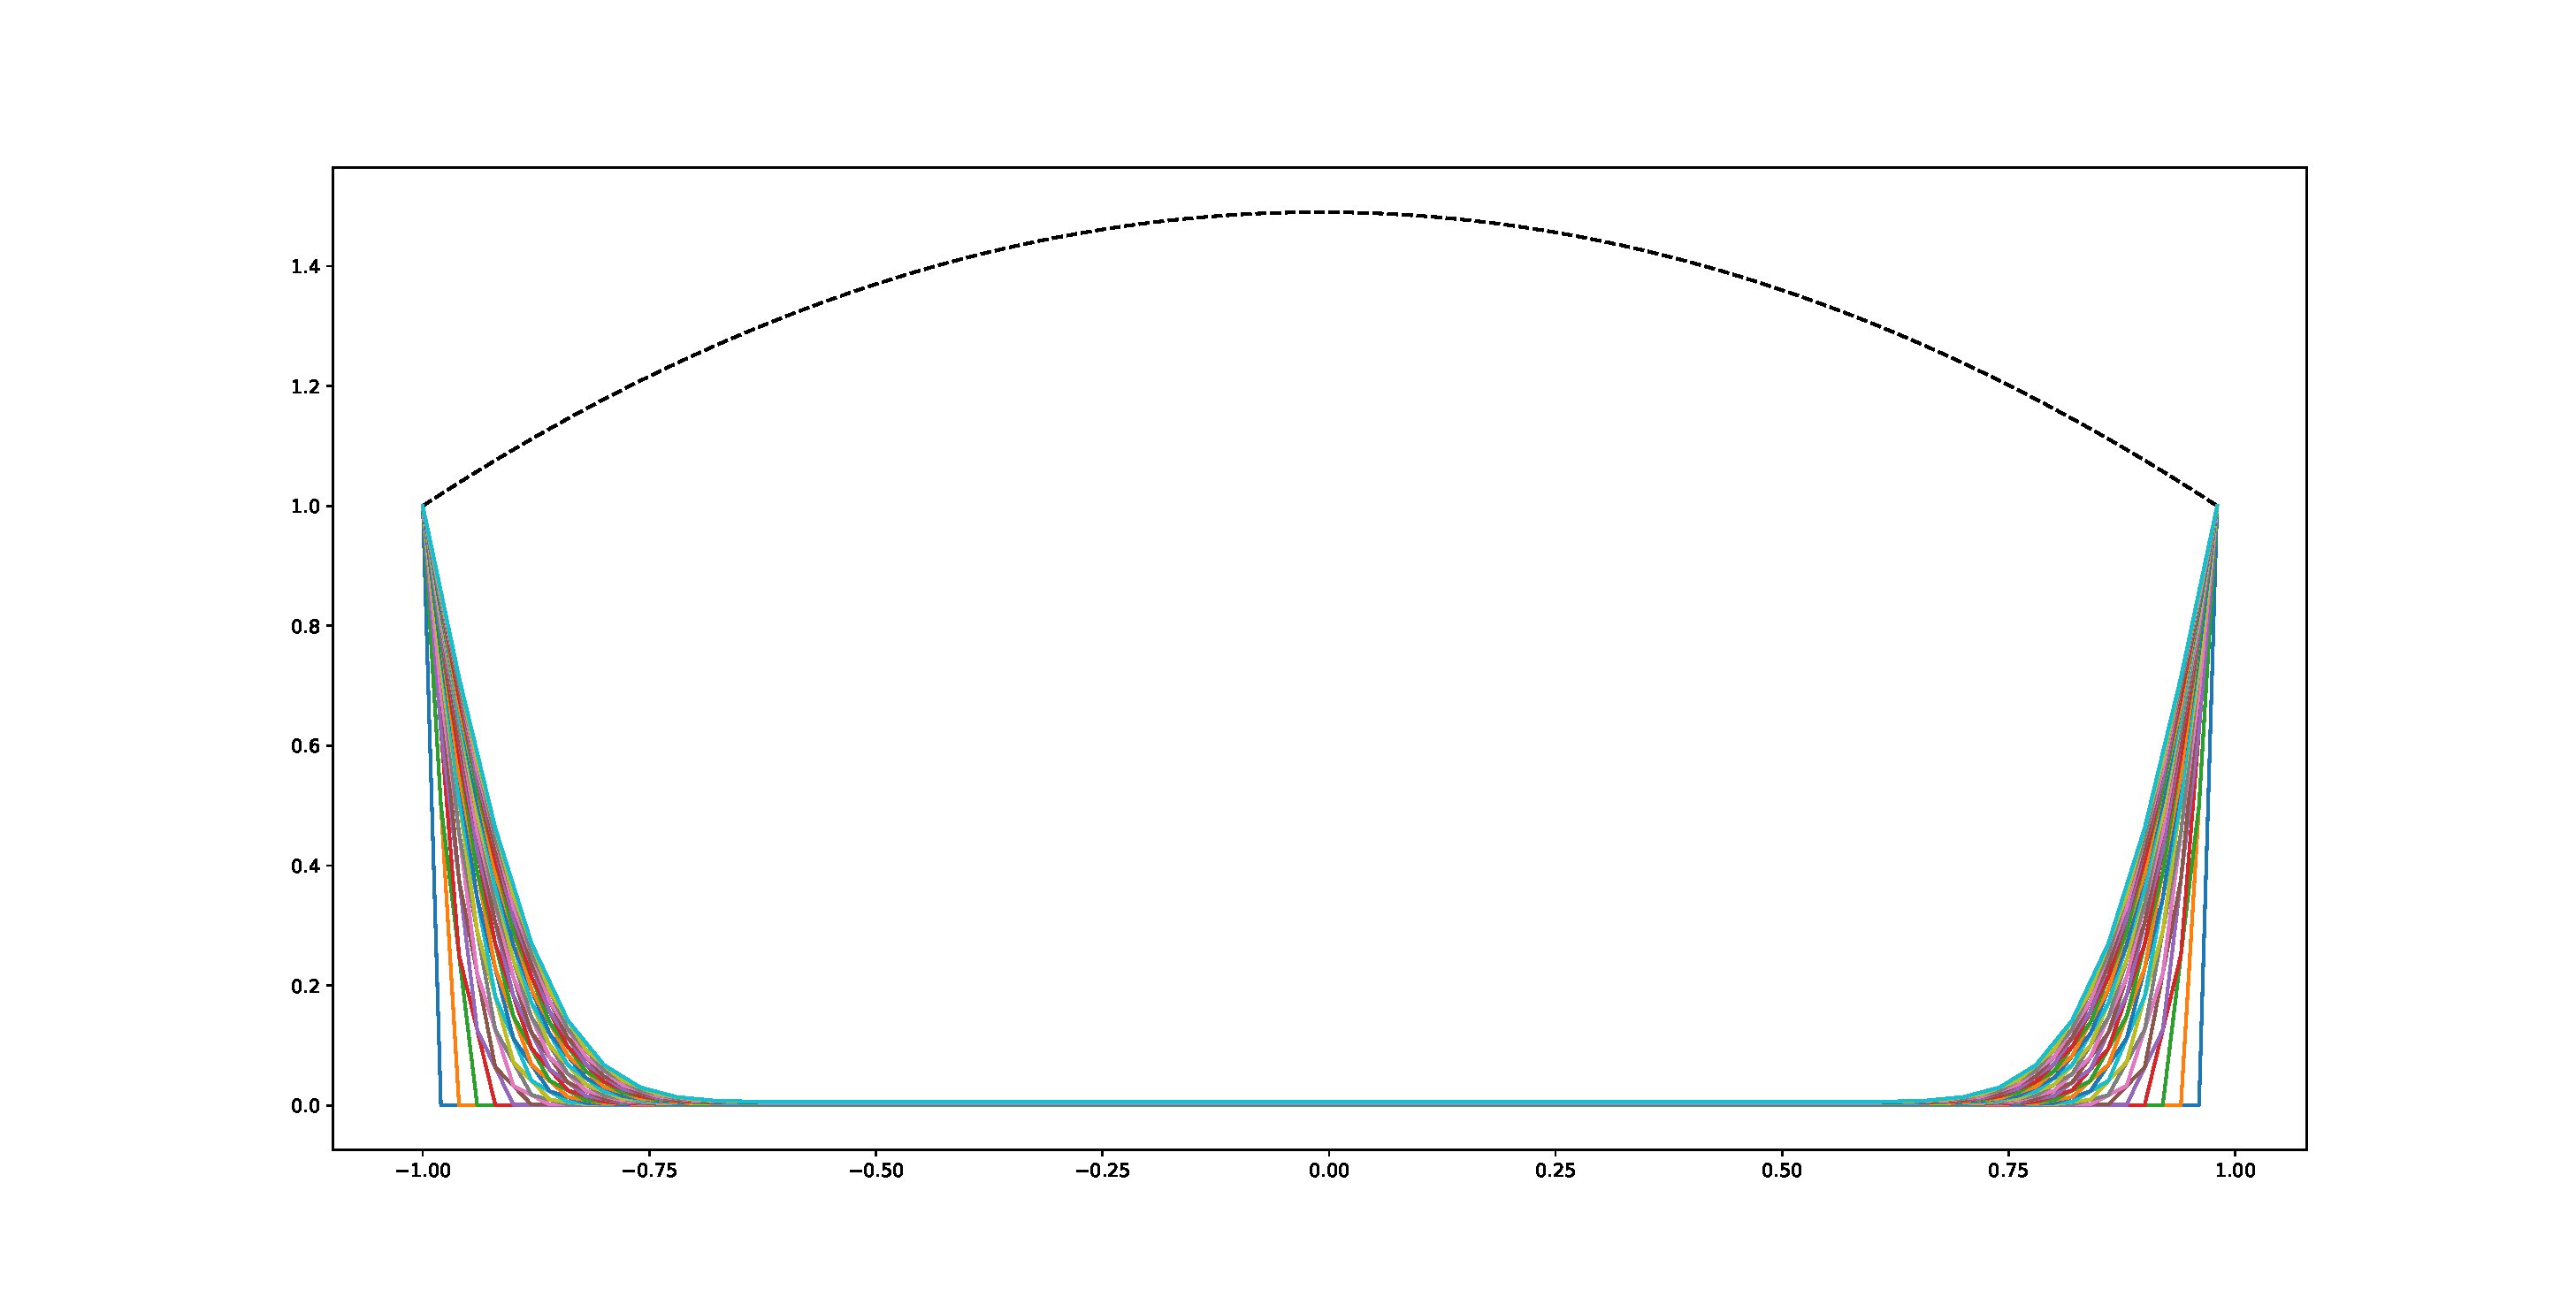
\includegraphics[width=1.1\linewidth]{Plots/Jacobi100.eps}
	\caption{Jacobi iteration for \(30\) steps and \( N=100 \). The black, dotted line indicates the solution obtained form he previous algorithm.}
	\label{fig:Jacobi100}
\end{figure}
Here, the solution does not converge to the expected parabola. This is due to the fact that the information from the boundaries can only travel 30 grid points in 30 steps because we have nearest neighbor coupling only. On a grid with 100 gridpoints the stepsize is thus not sufficiently large.

\subsection*{Exercise 1.2}

We begin with the construction of the restricted matrices. We employ a restriction scheme where the nearest neighbors are used to compute the coarser grid:
\begin{equation}
	x^{2h}_i = \frac{1}{4} x^{h}_{i-1} + \frac{1}{2} x^{h}_{i} + \frac{1}{4} x^{h}_{i+1}
\end{equation}
Writing this as a matrix for the \( 9 \times 5 \), the \( 5 \times 3\) and the \( 3 \times 2 \) case, we get:
\begin{equation}
	R_1 = \dfrac{1}{4}\begin{pmatrix}
	2&1&0&0&0&0&0&0&0\\
	0&1&2&1&0&0&0&0&0\\
	0&0&0&1&2&1&0&0&0\\
	0&0&0&0&0&1&2&1&0\\
	0&0&0&0&0&0&0&1&2
	\end{pmatrix}
\end{equation}
\begin{equation}
	R_2 = \dfrac{1}{4}\begin{pmatrix}
	2&1&0&0&0\\
	0&1&2&1&0\\
	0&0&0&1&2
	\end{pmatrix}
\end{equation}
\begin{equation}
	R_3 = \dfrac{1}{4}\begin{pmatrix}
	2&1&0\\
	0&1&2
	\end{pmatrix}
\end{equation}
We can do the same thing for the prolongation matrices with the mapping pattern that calculates the intermediate points as averages of the next points to the left and the right and maps the static points directly onto their counterpart on the finer grid.
\begin{align*}
	x_i^{h} = x_i{2h} \text{  if static point}\\
	x_i^{h} = \frac{1}{2}(x_{i+1}^{2h} + x_{i-1}^{2h})  \text{  if intermediate point}\\
\end{align*}
\begin{equation}
	P_0 = \dfrac{1}{2}\begin{pmatrix}
	2&0&0&0&0\\
	1&1&0&0&0\\
	0&2&0&0&0\\
	0&1&1&0&0\\
	0&0&2&0&0\\
	0&0&1&1&0\\
	0&0&0&2&0\\
	0&0&0&1&1\\
	0&0&0&0&2
	\end{pmatrix}
\end{equation}
\begin{equation}
	P_1 = \begin{pmatrix}
	2&0&0\\
	1&1&0\\
	0&2&0\\
	0&1&1\\
	0&0&2\\
	\end{pmatrix}
\end{equation}
\begin{equation}
	P_2 = \begin{pmatrix}
	2&0\\
	1&1\\
	0&2\\
	\end{pmatrix}
\end{equation}
We immediately see that the matrices are the transposed of the restriction matrices multiplied by a factor of 2.
\end{document}
